\documentclass[10pt]{article}
\usepackage[landscape, letterpaper, top=3cm, bottom=1.5cm, left=1.5cm, right=1.5cm]{geometry}
\usepackage{multicol}
\usepackage{fancyhdr}
\usepackage{lastpage}
\usepackage{listings}
\usepackage{xcolor}
\usepackage{titletoc}
\usepackage{hyperref}
\usepackage{graphicx}
\usepackage{tabularx}
\usepackage{ragged2e}
\usepackage{xltabular}
\usepackage{multirow}
\usepackage{amsmath}

% Configure column separation line
\setlength{\columnsep}{1cm}
\setlength{\columnseprule}{0.4pt}

% Compact C++ listing style
\lstdefinestyle{compactcpp}{
    language=C++,
    basicstyle=\ttfamily\footnotesize,
    keywordstyle=\color{blue},
    commentstyle=\color{green!50!black},
    stringstyle=\color{red},
    numbers=left,
    numberstyle=\tiny\color{gray},
    stepnumber=1,
    numbersep=3pt,
    backgroundcolor=\color{white},
    frame=single,
    framesep=1pt,
    rulecolor=\color{black!30},
    tabsize=4,
    showstringspaces=false,
    breaklines=true,
    belowskip=0pt,
    aboveskip=4pt
}

% Page style configuration
\pagestyle{fancy}
\fancyhf{}
\renewcommand{\headrulewidth}{0.4pt}
\renewcommand{\sectionmark}[1]{\markboth{#1}{}}
\fancyhead[L]{\authorname}
\fancyhead[C]{\leftmark}
\fancyhead[R]{Page \thepage\ of \pageref{LastPage}}
\fancyheadoffset{0pt}

% Author name definition
\newcommand{\authorname}{\textbf{Enrique Calderón, Luis Salazar, Gustavo Valenzuela}}

% Table of Contents formatting
\contentsmargin{0pt}
\dottedcontents{section}[1.5em]{}{2em}{1pc}
\dottedcontents{subsection}[3.8em]{}{2.8em}{1pc}

% Custom title page
\newcommand{\maketitlepage}{
    \begin{titlepage}
        \centering
        \vspace*{2cm}
        {\Huge\bfseries ICPC MX 2025 Reference\par}
        \vspace{1cm}
        {\Large \authorname \par}
        \vspace{2cm}
        {\large Last Updated: \today\par}
        \vfill
    \end{titlepage}
}

\begin{document}

% Title Page
\maketitlepage
\cleardoublepage

% Table of Contents Section
\section*{Table of Contents}
\begin{multicols*}{2}
    \startcontents[sections]
    \printcontents[sections]{l}{0}{\setcounter{tocdepth}{2}}
\end{multicols*}
\newpage

% Main Content
\begin{multicols*}{2}

\section{Data Types}
\begin{tabularx}{\linewidth}{|l|X|l|}
    \hline
    \textbf{Type} & \textbf{Range} & \textbf{Bytes} \\
    \hline
    bool & true or false & 1 bit \\
    \hline
    signed char & -128 to 127 & 1 \\
    \hline
    unsigned char & 0 to 255 & 1 \\
    \hline
    short int & -32,768 to 32,767 & 2 \\
    \hline
    unsigned short int & 0 to 65,535 & 2 \\
    \hline
    unsigned int & 0 to 4,294,967,295 & 4 \\
    \hline
    int & -2,147,483,648 to 2,147,483,647 & 4 \\
    \hline
    long int & -2,147,483,648 to 2,147,483,647 & 4 \\
    \hline
    unsigned long int & 0 to 4,294,967,295 & 4 \\
    \hline
    long long int & -(2\textasciicircum 63) to (2\textasciicircum 63)-1 & 8 \\
    \hline
    unsigned long long int & 0 to 18,446,744,073,709,551,615 & 8 \\
    \hline
    float & -3.4E38 to 3.4E38 & 4 \\
    \hline
    double & -1.7E308 to 1.7E308 & 8 \\
    \hline
    long double & -1.1E4932 to 1.1E4932 & 12 \\
    \hline
\end{tabularx}

\section{General algorithms}
\subsection{Sparse Table}
\subsubsection{Prerequisites}
\begin{itemize}
    \item Immutable array
    \item Associative function for O(n log n) range query
    \item Overlap friendly function O(1) range query (max, min, gcd, lcm)
\end{itemize}

\subsubsection{Implementation}
\begin{lstlisting}[style=compactcpp]
class SparseTable {
    vector<vector<int>> st;
    vector<int> logs;

public:
    SparseTable(vector<int>& arr) {
        int n = arr.size();
        int maxLog = 0;
        while ((1 << maxLog) <= n) maxLog++;

        st.assign(maxLog, vector<int>(n));
        logs.assign(n + 1, 0);

        // Precompute logs
        for (int i = 2; i <= n; i++) {
            logs[i] = logs[i / 2] + 1;
        }

        // Fill first row
        for (int i = 0; i < n; i++) {
            st[0][i] = arr[i];
        }

        // Fill table
        for (int j = 1; j < maxLog; j++) {
            for (int i = 0; i + (1 << j) <= n; i++) {
                st[j][i] = max(st[j-1][i], st[j-1][i + (1 << (j-1))]);
            }
        }
    }

    // O(1) range maximum query
    int query(int l, int r) {
        int j = logs[r - l + 1];
        return max(st[j][l], st[j][r - (1 << j) + 1]);
    }
};
\end{lstlisting}

\section{Geometry}

\subsection{Constants}
\subsubsection{PI}
\begin{lstlisting}[style=compactcpp]
#define PI acos(-1.0)
\end{lstlisting}

\subsubsection{Epsilon}
\begin{lstlisting}[style=compactcpp]
#define EPS 1e-9
\end{lstlisting}

\subsection{Conversions}
\subsubsection{Degree/Radian conversions}
\begin{lstlisting}[style=compactcpp]
double DEG_to_RAD(double d) { return d * PI / 180.0; }
double RAD_to_DEG(double r) { return r * 180.0 / PI; }
\end{lstlisting}

\subsection{Structures}
\subsubsection{Point}
\begin{lstlisting}[style=compactcpp]
struct point_i {
    int x, y;
    point_i() { x = y = 0; }
    point_i(int _x, int _y) : x(_x), y(_y) {}
};

struct point {
    double x, y;
    point() { x = y = 0.0; }
    point(double _x, double _y) : x(_x), y(_y) {}
};
\end{lstlisting}

\subsubsection{Line}
\begin{lstlisting}[style=compactcpp]
struct line {
    double a, b, c;
    // ax + by + c = 0
};
\end{lstlisting}

\subsection{Circle}
\subsubsection{Check if point is inside circle}
\begin{lstlisting}[style=compactcpp]
int insideCircle(point_i p, point_i c, int r) {
    int dx = p.x - c.x, dy = p.y - c.y;
    int Euc = dx * dx + dy * dy, rSq = r * r;
    return Euc < rSq ? 0 : Euc == rSq ? 1 : 2;
    // 0 = inside, 1 = on border, 2 = outside
}
\end{lstlisting}

\subsubsection{Arc Length}
To calculate the arc use \texttt{L = r * theta} where theta is in radians.

\subsection{Triangle}
\subsubsection{Area using Heron's formula}
\begin{lstlisting}[style=compactcpp]
double triangleArea(double a, double b, double c) {
    double s = (a + b + c) / 2.0; // semiperimeter
    return sqrt(s * (s - a) * (s - b) * (s - c));
}
\end{lstlisting}

\subsubsection{Distance between points}
\begin{lstlisting}[style=compactcpp]
double dist(point p1, point p2) {
    return sqrt((p1.x - p2.x) * (p1.x - p2.x) + (p1.y - p2.y) * (p1.y - p2.y));
}
\end{lstlisting}

\subsubsection{Perimeter}
\begin{lstlisting}[style=compactcpp]
double perimeter(double a, double b, double c) {
    return a + b + c;
}

double perimeter(point a, point b, point c) {
    return dist(a, b) + dist(b, c) + dist(c, a);
}
\end{lstlisting}

\subsection{Save int as real number}
For more precision you can use scanf:
\begin{lstlisting}[style=compactcpp]
int a, b;
scanf("%d.%d", &a, &b);
\end{lstlisting}

\section{C++ Functions}
\subsection{Common STL Algorithms}

\subsection*{Sorting Algorithms}
\begin{tabularx}{\linewidth}{|l|l|X|}
    \hline
    \textbf{Function} & \textbf{Parameters} & \textbf{Description} \\
    \hline
    sort & begin, end, [comp] & Standard unstable sort (O(n log n)) \\
    \hline
    stable\_sort & begin, end, [comp] & Stable sort preserves element order \\
    \hline
    is\_sorted & begin, end, [comp] & Checks if range is sorted (returns bool) \\
    \hline
    nth\_element & begin, nth, end, [comp] & Partitions around nth element \\
    \hline
\end{tabularx}

\subsection*{Searching Functions}
\begin{tabularx}{\linewidth}{|l|l|X|}
    \hline
    \textbf{Function} & \textbf{Parameters} & \textbf{Description} \\
    \hline
    lower\_bound & begin, end, val, [comp] & First element $\leq$ value \\
    \hline
    upper\_bound & begin, end, val, [comp] & First element > value \\
    \hline
    binary\_search & begin, end, val, [comp] & Existence check in sorted range \\
    \hline
    find & begin, end, val & Linear search for value \\
    \hline
    find\_if & begin, end, pred & Find first matching predicate \\
    \hline
\end{tabularx}

\subsection*{Sequence Operations}
\begin{tabularx}{\linewidth}{|l|l|X|}
    \hline
    \textbf{Function} & \textbf{Parameters} & \textbf{Description} \\
    \hline
    reverse & begin, end & Reverse elements in-place \\
    \hline
    rotate & begin, mid, end & Rotate elements left \\
    \hline
    next\_permutation & begin, end & Generate next permutation \\
    \hline
    unique & begin, end, [pred] & Remove consecutive duplicates \\
    \hline
    remove & begin, end, val & Remove elements equal to value \\
    \hline
\end{tabularx}

\subsection*{Numerical Functions}
\begin{tabularx}{\linewidth}{|l|l|X|}
    \hline
    \textbf{Function} & \textbf{Parameters} & \textbf{Description} \\
    \hline
    accumulate & begin, end, init, [op] & Sum/accumulate elements \\
    \hline
    partial\_sum & begin, end, dest, [op] & Compute prefix sums \\
    \hline
    \_\_gcd & a, b & Greatest common divisor (C++17) \\
    \hline
    lcm & a, b & Least common multiple (C++17) \\
    \hline
    iota & begin, end, val & Fill with consecutive values \\
    \hline
\end{tabularx}

\subsection*{Memory/Array Operations}
\begin{tabularx}{\linewidth}{|l|l|X|}
    \hline
    \textbf{Function} & \textbf{Parameters} & \textbf{Description} \\
    \hline
    memset & ptr, value, count & Fill memory with byte value \\
    \hline
    fill & begin, end, value & Fill range with value \\
    \hline
    fill\_n & begin, count, value & Fill N elements with value \\
    \hline
    copy & src\_b, src\_e, dest & Copy range to destination \\
    \hline
    copy\_if & src\_b, src\_e, dest, pred & Copy elements matching predicate \\
    \hline
\end{tabularx}

\subsection*{Utility Functions}
\begin{tabularx}{\linewidth}{|l|l|X|}
    \hline
    \textbf{Function} & \textbf{Parameters} & \textbf{Description} \\
    \hline
    swap & a, b & Swap two values \\
    \hline
    max\_element & begin, end, [comp] & Find maximum element \\
    \hline
    min\_element & begin, end, [comp] & Find minimum element \\
    \hline
    count & begin, end, val & Count element occurrences \\
    \hline
    all\_of & begin, end, pred & Check all elements satisfy condition \\
    \hline
\end{tabularx}

\subsection*{Mathematical / Bitwise Builtins}
\begin{tabularx}{\linewidth}{|l|l|X|}
    \hline
    \textbf{Function} & \textbf{Parameters} & \textbf{Description} \\
    \hline
    \_\_builtin\_popcount & x (int) & Count number of 1-bits \\
    \hline
    \_\_builtin\_popcountll & x (long long) & Count number of 1-bits (64-bit) \\
    \hline
    \_\_builtin\_clz & x (unsigned int) & Count leading zeros \\
    \hline
    \_\_builtin\_clzll & x (unsigned long long) & Leading zeros (64-bit) \\
    \hline
    \_\_builtin\_ctz & x (unsigned int) & Count trailing zeros \\
    \hline
    \_\_builtin\_ctzll & x (unsigned long long) & Trailing zeros (64-bit) \\
    \hline
    \_\_builtin\_parity & x & Return 1 if \#bits is odd \\
    \hline
    \_\_builtin\_ffs & x & Position of least significant 1-bit (1-indexed) \\
    \hline
    \_\_lg & x & Floor of $\log_2(x)$ (index of highest bit) \\
    \hline
\end{tabularx}

\subsection*{Priority Queues and Heaps}
\begin{tabularx}{\linewidth}{|l|l|X|}
    \hline
    \textbf{Function} & \textbf{Parameters} & \textbf{Description} \\
    \hline
    priority\_queue & [type], [container], [comp] & Max-heap by default \\
    \hline
    make\_heap & begin, end, [comp] & Turn range into heap \\
    \hline
    push\_heap & begin, end, [comp] & Push element into heap \\
    \hline
    pop\_heap & begin, end, [comp] & Pop max element into end \\
    \hline
    sort\_heap & begin, end, [comp] & Heap sort \\
    \hline
\end{tabularx}

\subsection*{Set / Map Utilities}
\begin{tabularx}{\linewidth}{|l|l|X|}
    \hline
    \textbf{Operation} & \textbf{Usage} & \textbf{Description} \\
    \hline
    s.lower\_bound(x) & set/map & First element $\geq$ x \\
    \hline
    s.upper\_bound(x) & set/map & First element $>$ x \\
    \hline
    s.equal\_range(x) & multiset/map & Pair of lower/upper bound \\
    \hline
    s.erase(it) & iterator & Erase element at iterator \\
    \hline
    s.find(x) & key & Iterator to key or end \\
    \hline
\end{tabularx}

\subsection*{String Functions}
\begin{tabularx}{\linewidth}{|l|l|X|}
    \hline
    \textbf{Function} & \textbf{Parameters} & \textbf{Description} \\
    \hline
    stoi, stol, stoll & string, [pos], [base] & Convert string $\to$ int/long/ll \\
    \hline
    stoul, stoull & string, [pos], [base] & Convert string $\to$ unsigned \\
    \hline
    stod, stof, stold & string & Convert string $\to$ double/float/long double \\
    \hline
    to\_string & value & Convert number $\to$ string \\
    \hline
    substr & pos, len & Substring \\
    \hline
    find & str, pos & Find first occurrence \\
    \hline
    rfind & str, pos & Find last occurrence \\
    \hline
\end{tabularx}

\subsection*{Random Number Utilities}
\begin{tabularx}{\linewidth}{|l|l|X|}
    \hline
    \textbf{Type / Function} & \textbf{Usage} & \textbf{Description} \\
    \hline
    mt19937 rng & chrono::steady\_clock::now() & Fast random generator \\
    \hline
    uniform\_int\_distribution & dist(a,b)(rng) & Random int in [a,b] \\
    \hline
    shuffle & begin, end, rng & Random shuffle \\
    \hline
\end{tabularx}

\subsection*{Other Useful Utilities}
\begin{tabularx}{\linewidth}{|l|l|X|}
    \hline
    \textbf{Function} & \textbf{Parameters} & \textbf{Description} \\
    \hline
    chrono::high\_resolution\_clock & now() & Get precise current time \\
    \hline
    \_\_int128 & value & 128-bit integer (manual I/O needed) \\
    \hline
    bitset<N> & ops: \&, |, \^, <<, >> & Fixed-size bitset manipulation \\
    \hline
    tuple & get$<i>$(t) & Store and access heterogenous data \\
    \hline
    pair & first, second & Store pair of values \\
    \hline
\end{tabularx}


\section{Binary search in the answer}
\lstinputlisting[style=compactcpp]{reference/binary_search/standard.cpp}
\section{Data Structures}
\subsection{Fenwick Tree}
\lstinputlisting[style=compactcpp]{reference/data_structures/fenwick_tree/fenwick_tree.cpp}

\subsection{Fenwick Minimum}
\lstinputlisting[style=compactcpp]{reference/data_structures/fenwick_tree/fenwick_min.cpp}

\subsection{1-Indexed Fenwick Tree}
\lstinputlisting[style=compactcpp]{reference/data_structures/fenwick_tree/fenwick_tree_one_based.cpp}

\subsection{Fenwick 2D (Sum query)}
\lstinputlisting[style=compactcpp]{reference/data_structures/fenwick_tree/fenwick_2d_sum.cpp}

\subsection{Fenwick 2D (Counting in range)}
\lstinputlisting[style=compactcpp]{reference/data_structures/fenwick_tree/fenwick_2d_counting.cpp}

\subsection{Fenwick Tree Range Update - Point Query}
\lstinputlisting[style=compactcpp]{reference/data_structures/fenwick_tree/fenwick_ruq.cpp}

\subsection{Fenwick Tree - Range update and query}
\lstinputlisting[style=compactcpp]{reference/data_structures/fenwick_tree/fenwick_rurq.cpp}

\subsection{Segment Tree (Iterative)}
\lstinputlisting[style=compactcpp]{reference/data_structures/segment_tree/segment_tree_iterative.cpp}

\subsection{Segment Tree (Sum query)}
\lstinputlisting[style=compactcpp]{reference/data_structures/segment_tree/segment_tree_sum.cpp}

\subsection{Segment Tree (Minimum query)}
\lstinputlisting[style=compactcpp]{reference/data_structures/segment_tree/segment_tree_min.cpp}

\subsection{Segment Tree Lazy Propagation}
\lstinputlisting[style=compactcpp]{reference/data_structures/segment_tree/segment_tree_lazy.cpp}

\subsection{Segment Tree 2D}
\lstinputlisting[style=compactcpp]{reference/data_structures/segment_tree/segment_tree_2d.cpp}

\subsection{Segment tree with Index Compression}
\lstinputlisting[style=compactcpp]{reference/data_structures/segment_tree/segment_tree_index_compression.cpp}

\subsection{Segment Tree Preffix-Suffix-Biggest}
\lstinputlisting[style=compactcpp]{reference/data_structures/segment_tree/segment_tree_psb.cpp}

\subsection{Persistent Array}
\lstinputlisting[style=compactcpp]{reference/data_structures/persistent/persistent_array.cpp}


\subsection{Path Copying - Persistent Array}
\lstinputlisting[style=compactcpp]{reference/data_structures/persistent/path_copying_persistent_array.cpp}

\subsection{Persistent Segment Tree}
\lstinputlisting[style=compactcpp]{reference/data_structures/persistent/persistent_segment_tree.cpp}

\subsection{Policy Ordered Set}
\lstinputlisting[style=compactcpp]{reference/data_structures/policy_ordered_set.cpp}

\subsection{Disjoint Set Union}
\lstinputlisting[style=compactcpp]{reference/data_structures/dsu/dsu.cpp}

\subsection{DSU to detect cycles}
\lstinputlisting[style=compactcpp]{reference/data_structures/dsu/dsu_cycle_detection.cpp}

\subsection{DSU to check online bipartitness}
\lstinputlisting[style=compactcpp]{reference/data_structures/dsu/dsu_bipartiteness.cpp}

\subsection{DSU with rollback}
\lstinputlisting[style=compactcpp]{reference/data_structures/dsu/dsu_with_rollback.cpp}

\subsection{Dynamic connectivity}
\lstinputlisting[style=compactcpp]{reference/data_structures/dsu/dynamic_connectivity.cpp}

\subsection{Trie}
\lstinputlisting[style=compactcpp]{reference/data_structures/trie/trie.cpp}

\subsection{Palindromic Tree}
\lstinputlisting[style=compactcpp]{reference/data_structures/trie/palindromic_tree.cpp}

\subsection{Implicit Treap}
\lstinputlisting[style=compactcpp]{reference/data_structures/treap/implicit_treap.cpp}

\subsection{Treap}
\lstinputlisting[style=compactcpp]{reference/data_structures/treap/treap.cpp}

% --------------------------------------------------------------------

\section{Graph Theory}

\subsection{Bipartite Check BFS}
\lstinputlisting[style=compactcpp]{reference/graph/bipartite_check_bfs.cpp}

\subsection{Cycle Detection DFS}
\lstinputlisting[style=compactcpp]{reference/graph/cycle_detection_dfs.cpp}

\subsection{Topological Sort}
\lstinputlisting[style=compactcpp]{reference/graph/topological_sort.cpp}

\subsection{Kahn's Algorithm}
\lstinputlisting[style=compactcpp,language=Python]{reference/graph/kahns_algorithm.py}

\subsection{Lexicographically Min. TopoSort}
\lstinputlisting[style=compactcpp]{reference/graph/lexicographically_min_toposort.cpp}

\subsection{BFS Flood Fill}
\lstinputlisting[style=compactcpp]{reference/graph/bfs_flood_fill.cpp}

\subsection{BFS Iterative Flood Fill}
\lstinputlisting[style=compactcpp]{reference/graph/bfs_iterative_flood_fill.cpp}

\subsection{DFS Flood Fill}
\lstinputlisting[style=compactcpp]{reference/graph/dfs_flood_fill.cpp}

\subsection{Lava Flow (Multi-source BFS)}
\lstinputlisting[style=compactcpp]{reference/graph/lava_flow.cpp}

\subsection{Dijkstra}
\lstinputlisting[style=compactcpp]{reference/graph/dijkstra.cpp}

\subsection{Bellman Ford (With path restoring)}
\lstinputlisting[style=compactcpp]{reference/graph/bellman_ford.cpp}

\subsection{SPFA Bellman Ford}
\lstinputlisting[style=compactcpp]{reference/graph/spfa.cpp}


\subsection{Floyd-Warshall}
\lstinputlisting[style=compactcpp]{reference/graph/floyd_warshall.cpp}

\subsection{Prim's Algorithm (MST)}
\lstinputlisting[style=compactcpp]{reference/graph/prim.cpp}

\subsection{Kruskal's Algorithm (MST)}
\lstinputlisting[style=compactcpp]{reference/graph/kruskal.cpp}

\subsection{Another Kruskal}
\lstinputlisting[style=compactcpp]{reference/graph/another_kruskal.cpp}

\subsection{Kosaraju Algorithm (SCC)}
\lstinputlisting[style=compactcpp]{reference/graph/kosaraju.cpp}

\subsection{SCC}
\lstinputlisting[style=compactcpp]{reference/graph/scc.cpp}

\subsection{Tarjan algorithm (SCC)}
\lstinputlisting[style=compactcpp]{reference/graph/tarjan_scc.cpp}

\subsection{Finding Articulation Points}
\lstinputlisting[style=compactcpp]{reference/graph/articulation_points.cpp}

\subsection{Finding bridges}
\lstinputlisting[style=compactcpp]{reference/graph/bridges.cpp}

\subsection{Finding Bridges Online}
\lstinputlisting[style=compactcpp]{reference/graph/bridges_online.cpp}

\subsection{Bridge Tree}
\lstinputlisting[style=compactcpp]{reference/graph/bridge_tree.cpp}


\subsection{2-SAT}
\lstinputlisting[style=compactcpp]{reference/graph/2_sat.cpp}

\subsection{Hierholzer's Algorithm (Eulerian Path)}
\lstinputlisting[style=compactcpp]{reference/graph/hierholzer.cpp}

\subsection{Gale-Shapley Algorithm (Stable marriage)}
\lstinputlisting[style=compactcpp]{reference/graph/gale_shapley.cpp}

\section{Trees}

\subsection{Succesor}
\lstinputlisting[style=compactcpp]{reference/trees/succesor.cpp}

\subsection{Euler Tour}
\lstinputlisting[style=compactcpp]{reference/trees/euler_tour.cpp}

\subsection{Lowest Common Ancestor}
\lstinputlisting[style=compactcpp]{reference/trees/lca.cpp}

\subsection{Binary Lifting}
\lstinputlisting[style=compactcpp]{reference/trees/binary_lifting.cpp}

\subsection{Cartesian Tree}
\lstinputlisting[style=compactcpp]{reference/trees/cartesian_tree.cpp}

\subsection{Heavy-Light Decomposition}
\lstinputlisting[style=compactcpp]{reference/trees/hld.cpp}

\subsection{Centroid Decomposition}
\lstinputlisting[style=compactcpp]{reference/trees/centroid_decomposition.cpp}

\subsection{Tree Distances}
\lstinputlisting[style=compactcpp]{reference/trees/tree_distances.cpp}

\section{Flows}

\subsection{Ford-Fulkerson Maximum Flow}
\lstinputlisting[style=compactcpp]{reference/flows/ford_fulkerson.cpp}

\subsection{Dinic's Max Flow}
\lstinputlisting[style=compactcpp]{reference/flows/dinic.cpp}

\subsection{Min-cost Flow}
\lstinputlisting[style=compactcpp]{reference/flows/min_cost_flow.cpp}

\subsection{Hungarian Algorithm}
\lstinputlisting[style=compactcpp]{reference/flows/hungarian.cpp}

\subsection{Kuhn's Algorithm}
\lstinputlisting[style=compactcpp]{reference/flows/kuhn.cpp}

\section{Dynamic Programming}

\subsection{Coin Problem (Count ways)}
\lstinputlisting[style=compactcpp]{reference/dp/coin_problem_count_ways.cpp}

\subsection{Coin Problem (Count sorted ways)}
\lstinputlisting[style=compactcpp]{reference/dp/coin_problem_count_sorted_ways.cpp}

\subsection{Coin Problem (Minimum)}
\lstinputlisting[style=compactcpp]{reference/dp/coin_problem_minimum.cpp}

\subsection{Counting paths}
\lstinputlisting[style=compactcpp]{reference/dp/counting_paths.cpp}

\subsection{Longest Increasing Subsequence}
\lstinputlisting[style=compactcpp]{reference/dp/lis.cpp}

\subsection{Length of LIS}
\lstinputlisting[style=compactcpp]{reference/dp/lis_length.cpp}

\subsection{Longest Common Subsequence}
\lstinputlisting[style=compactcpp]{reference/dp/lcs.cpp}

\subsection{Edit Distance}
\lstinputlisting[style=compactcpp]{reference/dp/edit_distance.cpp}

\subsection{Bitmask DP}
\lstinputlisting[style=compactcpp]{reference/dp/bitmask_dp.cpp}

\subsection{Digit DP}
\lstinputlisting[style=compactcpp]{reference/dp/digit_dp.cpp}

\subsection{Double DP}
\lstinputlisting[style=compactcpp]{reference/dp/double_dp.cpp}

\section{Math}

\subsection{Prime}
\lstinputlisting[style=compactcpp]{reference/math/prime.cpp}

\subsection{Miller Rabin}
\lstinputlisting[style=compactcpp]{reference/math/miller_rabin.cpp}

\subsection{Sieve of Erathostenes}
\lstinputlisting[style=compactcpp]{reference/math/sieve.cpp}

\subsection{Sieve of Eratosthenes (count primes)}
\lstinputlisting[style=compactcpp]{reference/math/sieve_count_primes.cpp}
\subsection{Segmented Sieve}
\lstinputlisting[style=compactcpp]{reference/math/segmented_sieve.cpp}
\subsection{Linear sieve}
\lstinputlisting[style=compactcpp]{reference/math/linear_sieve.cpp}

\subsection{Sum of divisors}
\lstinputlisting[style=compactcpp]{reference/math/sum_of_divisors.cpp}

\subsection{Finding the divisors of a number (Trial Division)}
\lstinputlisting[style=compactcpp]{reference/math/trial_division.cpp}

\subsection{Factorials}
\lstinputlisting[style=compactcpp]{reference/math/factorials.cpp}

\subsection{Binpow}
\lstinputlisting[style=compactcpp]{reference/math/binpow.cpp}
\subsection{Modulo Inverse}
\lstinputlisting[style=compactcpp]{reference/math/modulo_inverse.cpp}

\subsection{BinPow Modulo Inv}
\lstinputlisting[style=compactcpp]{reference/math/binpow_mod_inv.cpp}
\subsection{Binomial Coefficients}
\lstinputlisting[style=compactcpp]{reference/math/binomial_coefficients.cpp}
\subsection{Newton Method (Sqrt and iSqrt)}
\lstinputlisting[style=compactcpp]{reference/math/newton_method.cpp}
\subsection{Integration with Simpson Method}
\lstinputlisting[style=compactcpp]{reference/math/simpson_integration.cpp}
\subsection{Ternary Search}
\lstinputlisting[style=compactcpp]{reference/math/ternary_search.cpp}
\subsection{DP Pascal triangle 1D}
\lstinputlisting[style=compactcpp]{reference/math/dp_pascal_1d.cpp}
\subsection{DP Pascal triangle 2D}
\lstinputlisting[style=compactcpp]{reference/math/dp_pascal_2d.cpp}


\subsection{Euler's Totient}
\lstinputlisting[style=compactcpp]{reference/math/eulers_totient.cpp}

\subsection{Diophantine equations}
\lstinputlisting[style=compactcpp]{reference/math/diophantine_equations.cpp}

\subsection{Discrete Log}
\lstinputlisting[style=compactcpp]{reference/math/discrete_log.cpp}

\section{Polynomials}

\subsection{FFT}
\lstinputlisting[style=compactcpp]{reference/polynomials/fft.cpp}

\subsection{NTT}
\lstinputlisting[style=compactcpp]{reference/polynomials/ntt.cpp}

\subsection{Berlekamp Messey}
\lstinputlisting[style=compactcpp]{reference/polynomials/berlekamp_messey.cpp}

\section{Linear Algebra}

\subsection{Determinant of a Matrix}
\lstinputlisting[style=compactcpp]{reference/linear_algebra/determinant.cpp}

\subsection{Rank of a Matrix}
\lstinputlisting[style=compactcpp]{reference/linear_algebra/rank.cpp}


\subsection{Gauss-Jordan}
\lstinputlisting[style=compactcpp]{reference/linear_algebra/gauss_jordan.cpp}


\subsection{Matrix Exponentiation}
\lstinputlisting[style=compactcpp]{reference/linear_algebra/matrix_exponentiation.cpp}

\section{Geometry}

\subsection{Line Segment Intersection}
\lstinputlisting[style=compactcpp]{reference/geometry/line_segment_intersection.cpp}
\subsection{Minimum Euclidian Distance}
\lstinputlisting[style=compactcpp]{reference/geometry/min_euclidean_distance.cpp}
\subsection{Point in polygon}
\lstinputlisting[style=compactcpp]{reference/geometry/point_in_polygon.cpp}
\subsection{Point Location Test}
\lstinputlisting[style=compactcpp]{reference/geometry/point_location_test.cpp}
\subsection{Polygon Area}
\lstinputlisting[style=compactcpp]{reference/geometry/polygon_area.cpp}
\subsection{Convex Hull}
\lstinputlisting[style=compactcpp]{reference/geometry/convex_hull.cpp}

\subsection{Complex point}
\lstinputlisting[style=compactcpp]{reference/geometry/complex_point.cpp}

\subsection{Polar sort}
\lstinputlisting[style=compactcpp]{reference/geometry/polar_sort.cpp}

\section{Strings}

\subsection{Marranadas de Quique}
\lstinputlisting[style=compactcpp]{reference/strings/marranadas_de_quique.cpp}

\subsection{KMP Algorithm}
\lstinputlisting[style=compactcpp]{reference/strings/kmp.cpp}

\subsection{Rolling Hash}
\lstinputlisting[style=compactcpp]{reference/strings/rolling_hash.cpp}

\subsection{Hash marrano}
\lstinputlisting[style=compactcpp]{reference/strings/hash_marrano.cpp}

\subsection{Suffix Array}
\lstinputlisting[style=compactcpp]{reference/strings/suffix_array.cpp}

\subsection{LCP}
\lstinputlisting[style=compactcpp]{reference/strings/lcp.cpp}

\subsection{Z Function}
\lstinputlisting[style=compactcpp]{reference/strings/z_function.cpp}

\subsection{Longest Palindrome}
\lstinputlisting[style=compactcpp]{reference/strings/longest_palindrome.cpp}

\subsection{String Hashing}
\lstinputlisting[style=compactcpp]{reference/strings/string_hashing.cpp}

\subsection{Manacher Algorithm}
\lstinputlisting[style=compactcpp]{reference/strings/manacher.cpp}

\subsection{Suffix Automaton}
\lstinputlisting[style=compactcpp]{reference/strings/suffix_automaton.cpp}
\section{Formulas}

\subsection{Sums}

\[
c^a+c^{a+1}+\dots + c^b = \frac{c^{b+1}-c^a}{c-1}, c\neq 1
\]

\textbf{Gauss}

\[
1+2+3+...+n = \frac{n(n+1)}{2}
\]

\textbf{Gauss squares}

\[
1^2+2^2+3^2+...+n^2 = \frac{n(2n+1)(n+1)}{6}
\]

\textbf{Cubes}

\[
1^3+2^3+3^3+...+n^3 = \frac{n^2(n+1)^2}{4}
\]

\textbf{Powers of 4}

\[
1^4+2^4+3^4+...+n^4 = \frac{n(2n+1)(n+1)(3n^2+3n-1)}{30}
\]

\subsection{Catalan numbers}
\[
C_0 = 1, \quad C_{n+1} = \sum_{i=0}^{n} C_i C_{n-i} \quad \text{(Recursive)}
\]
\[
C_n = \frac{1}{n+1} \binom{2n}{n} = \binom{2n}{n} - \binom{2n}{n+1} = \frac{(2n)!}{(n+1)!n!} \quad \text{(Closed-form)}
\]

\begin{itemize}
    \item \textbf{Valid Parentheses}: Count of balanced parentheses expressions with \( n \) pairs.
    \item \textbf{Full Binary Trees}: Structurally unique full binary trees with \( n+1 \) leaves.
    \item \textbf{Polygon Triangulation}: Ways to triangulate a convex \( (n+2) \)-gon.
    \item \textbf{Dyck Paths}: Paths from \( (0,0) \) to \( (2n,0) \) that never dip below the x-axis.
    \item \textbf{Non-Crossing Partitions}: Ways to connect \( 2n \) points on a circle without crossing chords.
    \item \textbf{Stack Permutations}: Valid stack-sortable permutations of length \( n \).
    \item \textbf{Mountain Ranges}: Sequences of \( 2n \) up/down steps forming valid mountain ranges.
    \item \textbf{Unique BSTs}: Number of distinct binary search trees with \( n \) keys.
    \item \textbf{Diagonal-Avoiding Paths}: Paths in a grid from \( (0,0) \) to \( (n,n) \) without crossing the diagonal.
\end{itemize}

\subsection{Cayley's Formula}

Number of labeled trees of n vertices: $n^{n-2}$.

Number of rooted forest of n vertices is: $(n+1)^{n-1}$

\subsection{Geometric series}

% Finite Geometric Series
\textbf{Finite:} \[\quad \sum_{k=0}^{n} ar^k = 
\begin{cases} 
a \dfrac{1 - r^{n+1}}{1 - r} & \text{if } r \neq 1, \\
a(n + 1) & \text{if } r = 1.
\end{cases}
\]
% Infinite Geometric Series
\textbf{Infinite:} \[\quad \sum_{k=0}^{\infty} ar^k = \frac{a}{1 - r} \quad \text{(converges iff } |r| < 1\text{)}
\]
\subsection{Divisors}

The number of divisors of any number n is:

\[
\begin{cases}
    \approx 100 \quad n< 5 \times 10^4 \\
    \approx 500 \quad n<1 \times 10^7 \\
    \approx 2000 \quad n < 1 \times 10^10 \\
    \approx 200000 \quad n < 1 \times 10^19
\end{cases}
\]

\subsection{Number of primes between 1 and n}

\[
\frac{n}{ln(n)}
\]


\subsection{Pythagorean triplets}

\[
a = k \cdot (m^2 - n^2), \quad b = k\cdot(2mn), \quad c = k\cdot(m^2+n^2)
\]

With $m>n>0$, $k=0$, $m\perp n$, and either m or n even.


\subsection{Derangments}

Permutations of a set sush that none of the elements appear in their original position.

\[
D(n) = (n-1)(D(n-1)+D(n-2)) = nD(n-1)+(-1)^n = \lfloor \frac{n!}{e}\rfloor
\]

\section{Miscellaneous}

\subsection{Implementation tricks}
\lstinputlisting[style=compactcpp]{reference/misc/implementation_tricks.cpp}

\subsection{Get Least Significant Bit}
\lstinputlisting[style=compactcpp]{reference/misc/lsb.cpp}

\subsection{Is power of two?}
\lstinputlisting[style=compactcpp]{reference/misc/is_power_of_two.cpp}

\subsection{Random number generator}
\lstinputlisting[style=compactcpp]{reference/misc/random_number_generator.cpp}

\subsection{Custom comparators}
\lstinputlisting[style=compactcpp]{reference/misc/custom_comparators.cpp}

\subsection{Kadane's Algorithm}
\lstinputlisting[style=compactcpp]{reference/misc/kadanes_algorithm.cpp}

\subsection{Moore's Voting Algorithm}
\lstinputlisting[style=compactcpp]{reference/misc/moores_voting_algorithm.cpp}

\subsection{ASCII table}
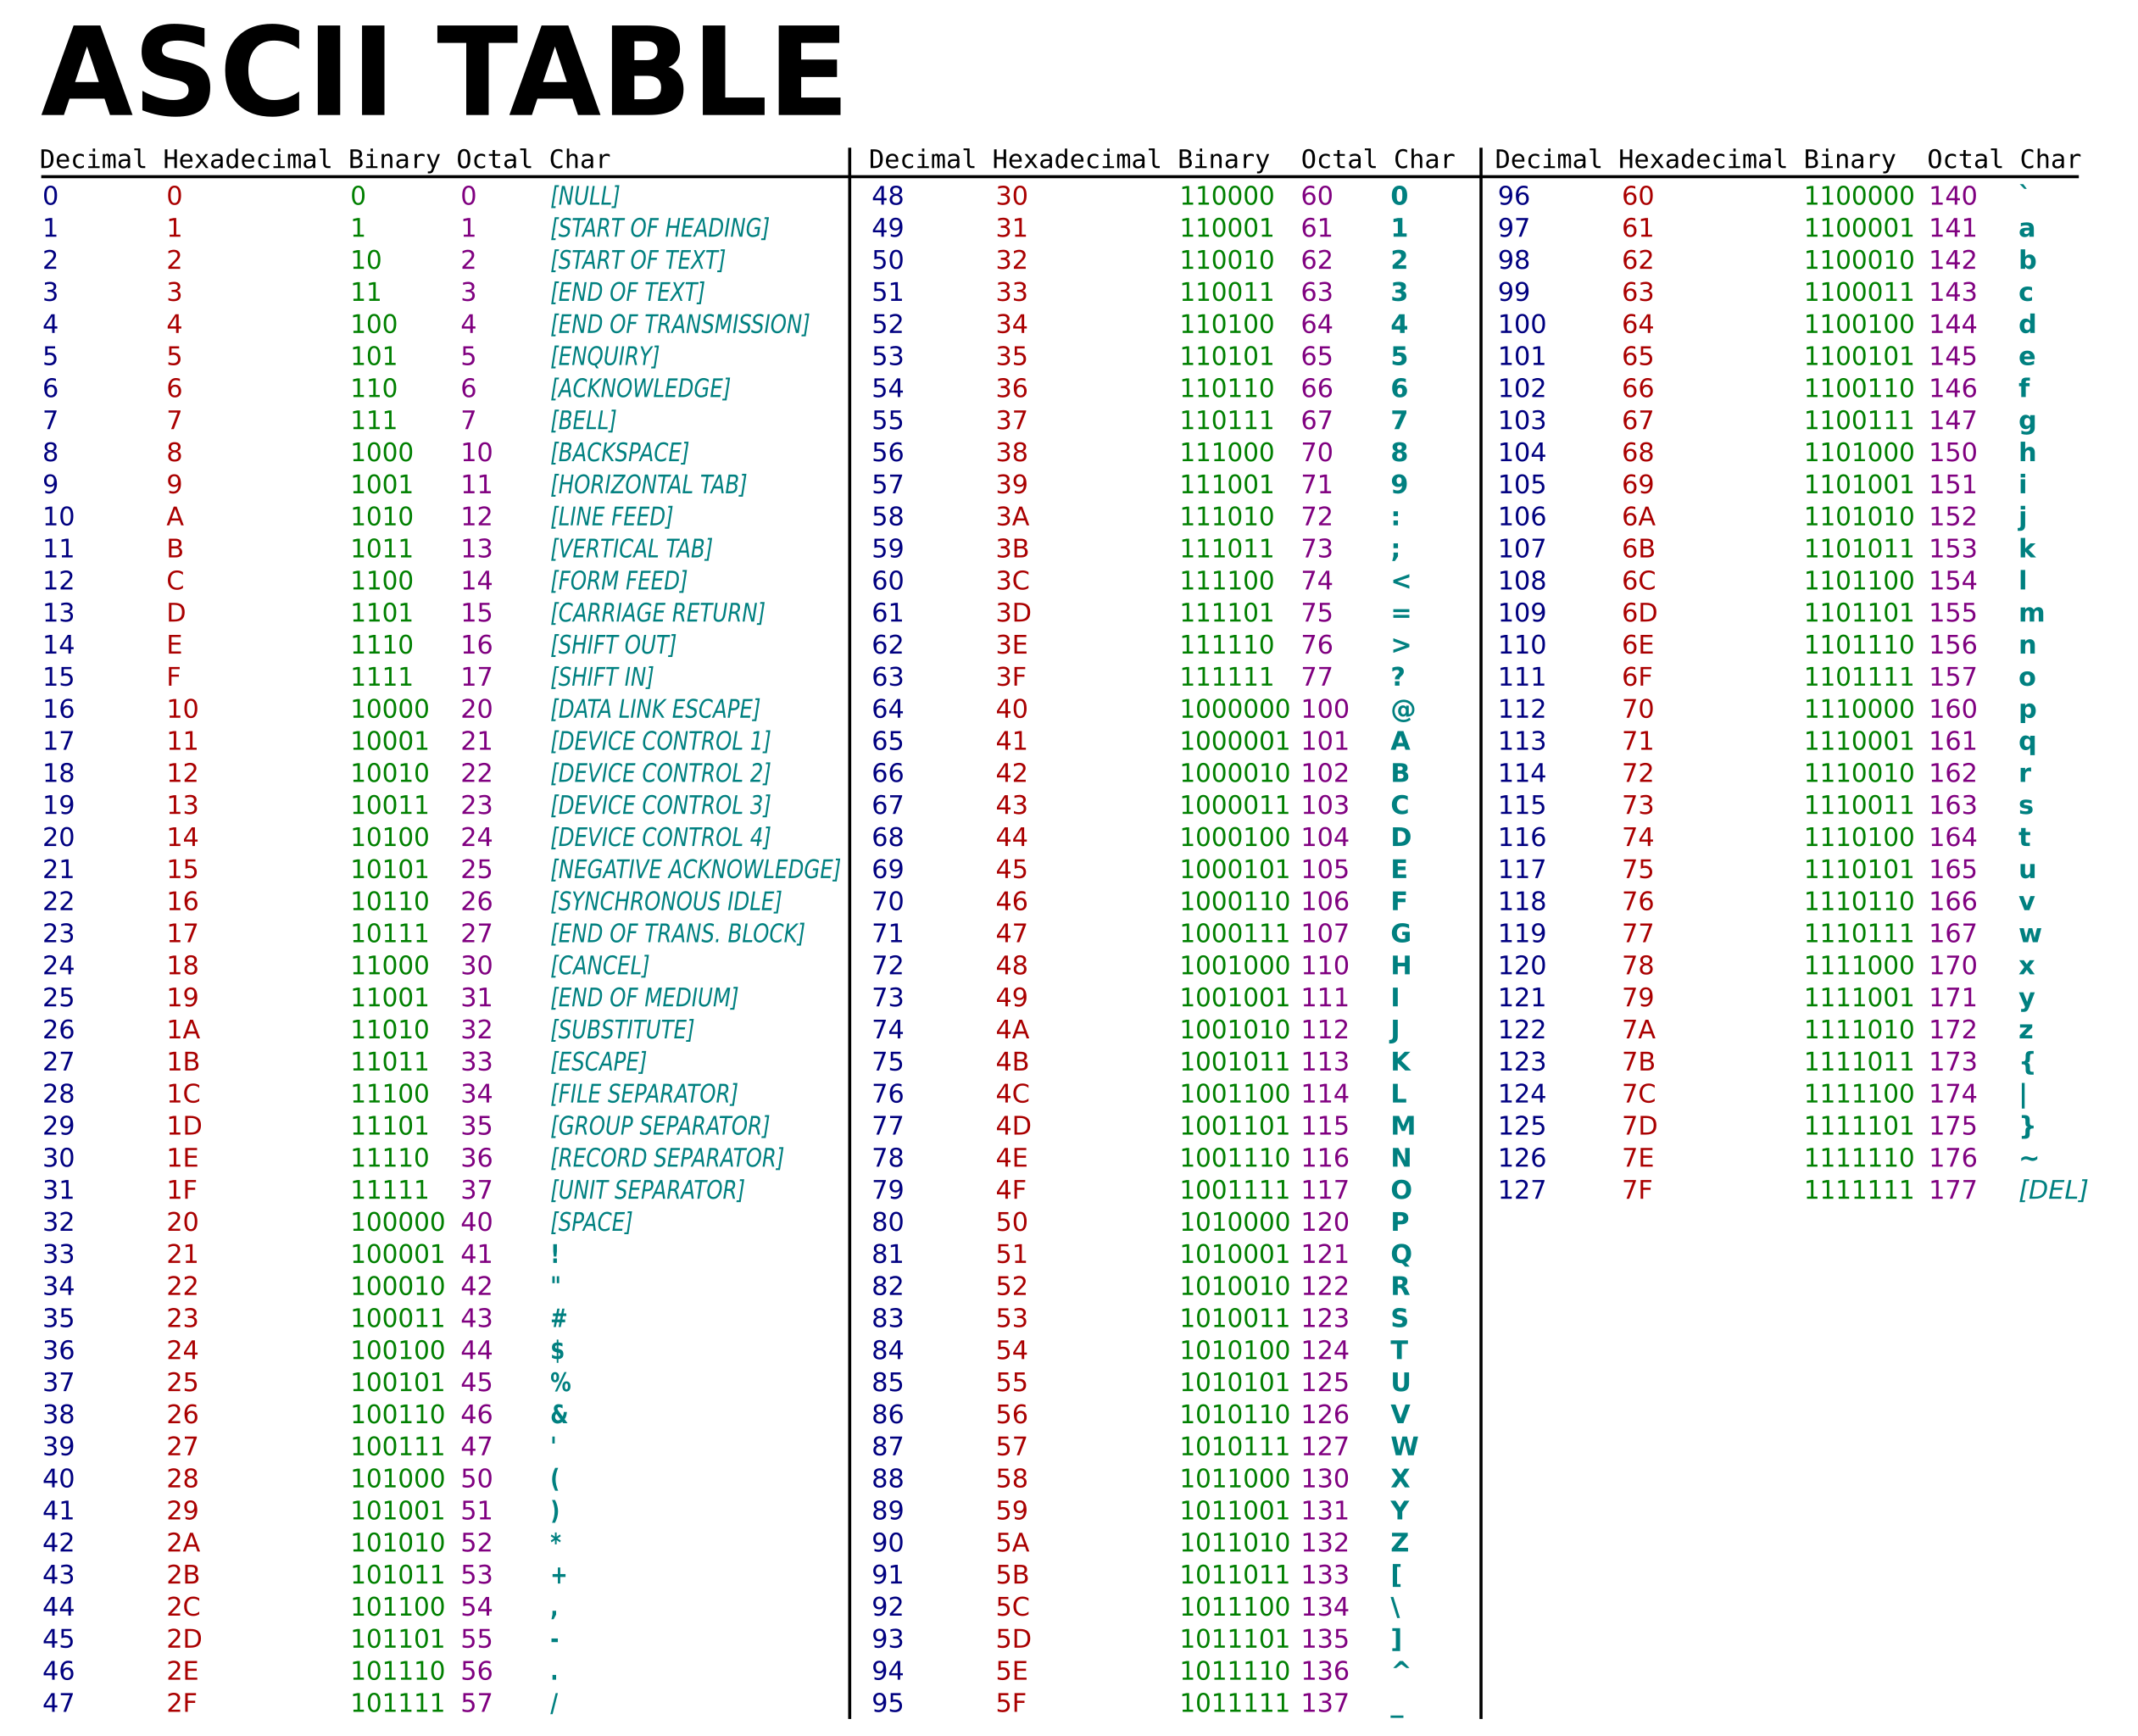
\includegraphics[width=0.8\linewidth]{img/ASCII-Table.png}

\section{C++ stuff}

\subsection{Compilation}

\texttt{g++-13 -std=c++20 name.cpp}

\subsection{Compiler optimizations}


\begin{lstlisting}[style=compactcpp]
// Makes bit operations faster
#pragma GCC target("popcnt") 

//Auto vectorize for-loops and optimizes floating points (assumes associativity and turns off denormals)
#pragma GCC optimize("Ofast")

// Doubles performance of vectorized code, crashes in old computers
#pragma GCC target("avx2")

#pragma GCC optimize("O3,unroll-loops")
#pragma GCC target("avx2,bmi,bmi2,lzcnt,popcnt")
\end{lstlisting}

\subsection{Decimal printing}

Friendly reminder to use \texttt{printf()} with decimals

\begin{lstlisting}[style=compactcpp]
cout<< fixed << setprecision(n)<<endl;
\end{lstlisting}

\subsection{Bit tricks}

x \& -x is the least bit in x

c = x \& -x, r=x+c, \texttt{(((bin\_pow(r,x)) >> 2)/c) OR r}  next number bigger than x same number of bits set.

\end{multicols*}


\end{document}